\subsection*{Q1}
\addcontentsline{toc}{subsection}{Q1} 
\begin{enumerate}[label=\alph*]
    \item In CT images it is easy to differentiate different types of soft tissues.
    \subitem False, soft tissues have a similar effective attenuation coefficient. Therefore, it is not easy to distinguish between soft tissues, but soft and hard tissue.
    \item There are no biological hazards due to x-ray exposure.
    \subitem False, due to the high energy of x-ray beams, which causes ionization of tissue, the biological risk is of a mutagenic resp. cancerogenic manner.
    \item The 2D Fourier transform of the image can be obtained from the acquired sinogram.
    \subitem True, the Fourier slice theorem specifies exactly this issue.
   % \begin{equation*}
%        \mu (x,y) = \frac{1}{4\pi^2}\int_{0}^{2 \pi} %{\int_{-\infty}^{+\infty}{\frac{1}{-x \sin{\theta} + y \cos{\theta} - s}\  %\frac{\partial R(\theta,s)}{\partial s}ds d\theta}}
%    \end{equation*}
    \item No representative images are rendered with back-projection when the views are not filtered.
    \subitem True, in order to enhance the contrast of features in the picture you have to filter it, though.
    \item The total attenuation of a non-monochromatic x-ray beam increases linearly with depth for a uniform medium.
    \subitem True,
    \begin{equation}
        \textbf{I} = I_0\ e^{-\mu_1 L_1} e^{-\mu_2 L_2} e^{-\mu_3 L_3} = I_0 e^{\underbrace{-\mu_1 L_1 -\mu_2 L_2- \mu_3 L_3}_{\text{\normalfont linear terms}}}
    \end{equation}    
\end{enumerate}

\subsection*{Q2}
\addcontentsline{toc}{subsection}{Q2} 
\subsubsection*{a}
\addcontentsline{toc}{subsubsection}{a} 
\begin{figure}[!htb]
    \centering
    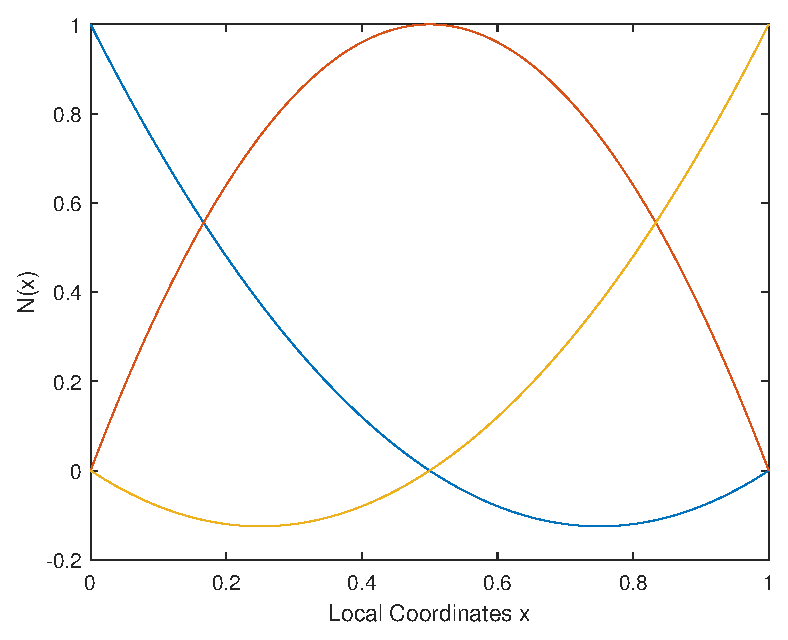
\includegraphics[width=.4\linewidth]{./midterm/img/3.eps}
    \caption{Signal shape at 0\textdegree}
    \label{fig:0}
\end{figure}
\begin{figure}[!htb]
    \centering
    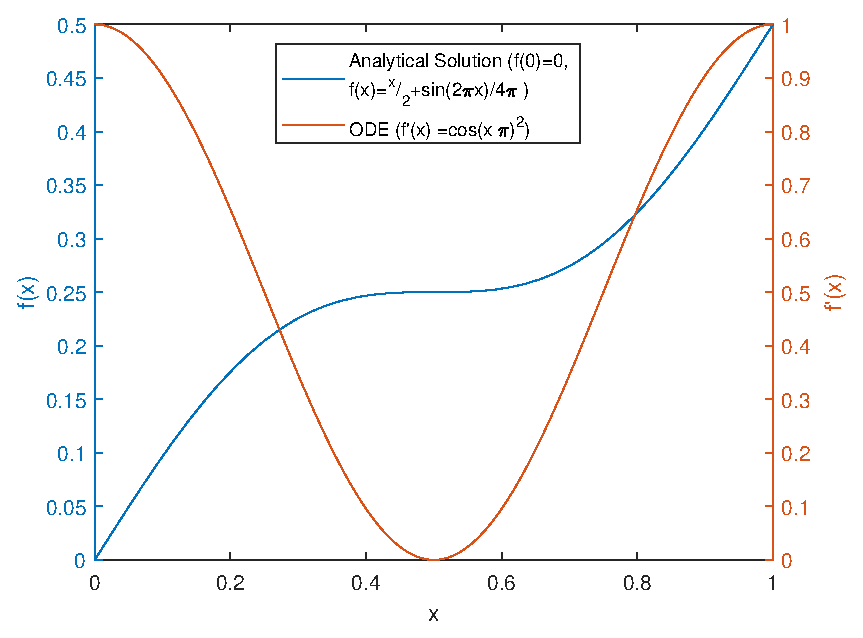
\includegraphics[width=.4\linewidth]{./midterm/img/1.eps}
    \caption{Signal shape at 45\textdegree}
    \label{fig:45}
\end{figure}
\begin{figure}[!htb]
    \centering
    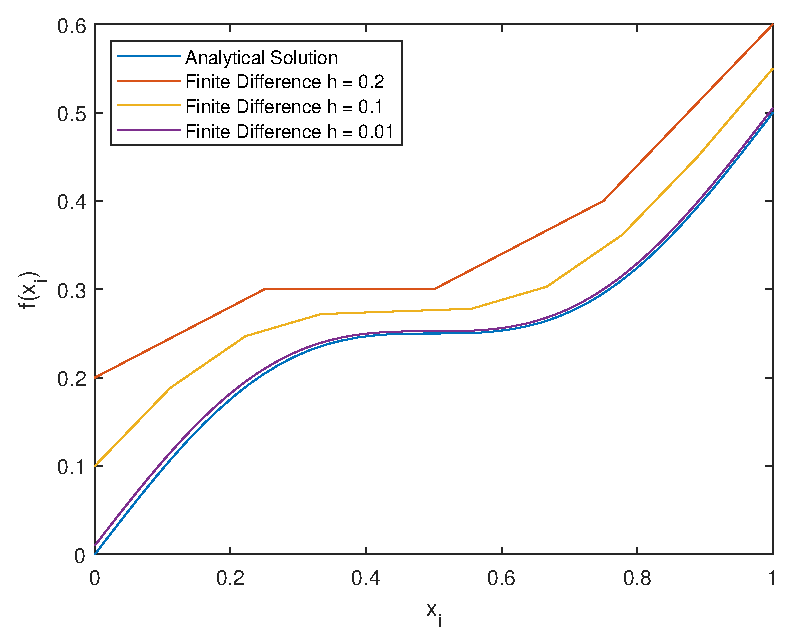
\includegraphics[width=.4\linewidth]{./midterm/img/2.eps}
    \caption{Signal shape at 90\textdegree}
    \label{fig:90}
\end{figure}
\clearpage
\subsubsection*{b}
\addcontentsline{toc}{subsubsection}{b} 
As seen in the figures \ref{fig:0},\ref{fig:45} and \ref{fig:90}, the highest peak of the accumulated intensity is at the signal from 45\textdegree. The position of $2\sqrt{2}$ on the x-axis of plot \ref{fig:45} corresponds thereby to the complete diagonal ray from the lower left to the upper right corner in the lower scheme (Fig. \ref{fig:perfect_ray}).
\begin{figure}[!htb]
    \centering
    \includegraphics[clip,width=.6\linewidth,trim=9mm 0mm 115mm 13mm]{./midterm/img/Rays.png}
    \caption{Perfect Ray}
    \label{fig:perfect_ray}
\end{figure}



\subsection*{Q3}
\addcontentsline{toc}{subsection}{Q3} 
Calculate resolution of an optical microscope given the following characteristics:
\begin{itemize}
    \item Magnification $\textbf{M}$ = 60x
    \item Lens Diameter $\textbf{D}$ = \SI{9.4}{\milli\meter}
    \item Focal Length $\textbf{f}$ = \SI{2.4}{\mm}
    \item Immersion Medium: oil, $\textbf{n}$ = 1.33
    \item Illumination \boldmath$\lambda$ = \SI{560}{\nm}
\end{itemize}

\begin{align}
    d &= \frac{\lambda}{2 \mathrm{NA}} \\
    &= \frac{\lambda}{2 n \sin{\theta}} \\
    &= \frac{\lambda}{2 n \Big(\frac{0.5 D}{\sqrt{(0.5 D)^2 + f^2}}\Big)}\\
    &= \frac{\SI{560}{\nano\meter}}{2\ \cdot\ \num{1.33}\ \cdot\ \Big(\frac{0.5 \cdot \SI{9.4}{\mm}}{\sqrt{(0.5 \SI{9.4}{\mm})^2 + (\SI{2.9}{\mm}^2}}\Big)}\\
    &= \SI{0.25}{\micro\meter}
\end{align}

\subsection*{Q4}
\addcontentsline{toc}{subsection}{Q4} 
Which parameters influence the depth (slice thickness) that can be efficiently visualized by an optical microscope? How could high resolution images of thicker slices be obtained by a conventional microscope?
\\[2\baselineskip]
The main parameter to influence the penetration into the sample is the scattering inside. Furthermore, the wavelength and light intensity are also crucial physical parameters. At the optical microscope Numerical Aperture (resp. the diffraction), the optical density and reflectance of the sample influence imaging.\\
To overcome these hurdles an increase in NA resp. light intensity and/or a decrease in wavelength could yield more resolution. Generally speaking, the the overall diffraction limit (Abbe) has to be maxed out.


\subsection*{Q5}
\addcontentsline{toc}{subsection}{Q5} 
\begin{enumerate}[label=\alph*]
    \item The width of a signal in the time domain is proportional to the width in the frequency domain.
    \subitem True, the width in time domain is indirect proportional to a signal in the frequency domain. 
    \item The central pixel in the 2D k-space (k$_x$=0,k$_y$=0) corresponds to a uniform image in the space domain.
    \subitem True, the center of  the 2D k-space is a uniform image. One pixel corresponds to a constant picture frequency which means a uniform image in the space domain.
    \item A one-dimensional wave characterized by $u = u_0 \cos(−5x+3t−2.5)$ propagates towards the negative x direction.
    \subitem False, it propagates in the positive x-Direction (+3t Term)
    \item Deconvolution is particularly suited for systems with a narrow frequency response.
    \subitem True, a narrow frequency response implies that the image possesses only few strong gradients and therefore the image has poor feature edge quality. A deconvolution then sharpens the image.
    \item For a given aperture, diffraction is more prominent in the ultraviolet than in the infrared. 
    \subitem False, diffraction increases with increasing wavelength. The focal size of a microscope is ultimately diffraction limited and proportional to the wavelength.
    \begin{equation}
        d =\frac{\lambda}{2NA}
    \end{equation}
\end{enumerate}


\subsection*{Q6}
\addcontentsline{toc}{subsection}{Q6} 
For a diffuse medium with prominent Rayleigh scattering, provide the wavelength dependence of the effective attenuation coefficient in a spectral range where the absorption coefficient increases linearly with wavelength.\\
Effective Attenuation Coefficient:\\
\begin{align}
    \mu_{eff} &= \sqrt{\frac{\mu_a}{D}},\ \mathrm{with}\ D = \frac{1}{3(\mu_a + \mu_s(1-g)},\ \mathrm{with}\ g \in [0.65,0.95] \\
    &= \sqrt{\mu_a\ \cdot\ 3(\mu_a + \mu_s(1-g))}
\end{align}
According the diffusion approximation that can be applied to solve the RTE scattering events are dominant over the absorption $\mu_s \gg \mu_a$. We therefore neglect the additive $\mu_a$.\\
Furthermore, Rayleigh scattering effects are dominant over others, which simplifies the equation according to $\mu_s \propto \lambda^{-4}$. With the wavelength dependence of the absorption coefficient $\mu_a \propto \lambda$, this leads to:
\begin{align}
\mu_{eff} &= \sqrt{3\mu_a\mu_s(1-g)}\\
&= \sqrt{3\lambda\lambda^{-4}(1-g)}\\
\Rightarrow \mu_{eff} &\propto \lambda^{-3/2}
\end{align}

\subsection*{Q7}
\addcontentsline{toc}{subsection}{Q7} 
An ideal camera moves in the x direction with constant velocity $\nu$ during exposure. If the exposure time is $\nu$ derive an expression for the point spread function and the transfer function of the imaging system. Demonstrate the effect of such motion on an image of your choice, assuming that $\nu T$ = 10 pixels. Provide Matlab code.

The PSF can be computed by:
\begin{equation}
f(x,y) = \begin{cases} \frac{1}{v\ T_{end}}, &for\ 0 \leq x \leq v T_{end} \\ 0, &otherwise \end{cases}
\end{equation}
Then, the images are overlapped along the interval by tranlation of the original picture.
\begin{lstlisting}
vT = 10;
img_orig = importdata('lena_full.png');
img = img_orig/(vT+1);
for i = 1:vT
    img = img + imtranslate(img_orig/(vT+1),[i 0]);
end
figure;
imshow(img_orig);
figure;
imshow(img);
imwrite(img,'lena_blurry.png');
\end{lstlisting}

\begin{figure}[htb!]
\begin{subfigure}[c]{0.5\linewidth}
\centering
\includegraphics[clip, trim=0 0mm 0 0,width=0.8\linewidth]{./midterm/img/lena_full.png}
\subcaption{Original Figure}
\end{subfigure}
\begin{subfigure}[c]{0.5\linewidth}
\centering
\includegraphics[clip, trim=0 0mm 0 0,width=0.8\linewidth]{./midterm/img/lena_blurry.png}
\subcaption{Blurry Picture}
\end{subfigure}

\caption{Pictures before and after processing}
\end{figure}

\subsection*{Q8}
\addcontentsline{toc}{subsection}{Q8} 
An infinitely large non absorbing medium with a high concentration of small spherical scatters is irradiated with blue, yellow and red light. Which beam penetrates deeper? Why? Give an analytical explanation.
\\[2\baselineskip]
As shown in the Planck-Einstein-Relation $E=h\frac{c}{\lambda}$, the light with low wavelength contains more energy than light with higher wavelengths. Therefore, photons with high energy scatter more often in tissue than photons with lower energy. Hence, even with anisotropic scattering high-energy photons pass more times the mean free path between to scattering events than low-energy photons.


\subsection*{Q9}
\addcontentsline{toc}{subsection}{Q9} 
Derive central, forward and backward finite difference approximations for the second order derivative $f''(x)$ of a function of one variable $f(x)$ ?
What is the truncation error of the derived approximations?\\
Forward Difference:\\
\begin{align}
    f'(x) &\approx \frac{f(x+h) -f(x)}{h}\\
    Then,\    f''(x) &\approx \frac{f'(x+h)-f'(x)}{h}\\
    &=\frac{\frac{f(x+2h)-f(x+h)}{h}-\frac{f(x+h)-f(x)}{h}}{h}\\
    &=\frac{f(x+2h)-2f(x+h)+f(x)}{h^2}
\end{align}
Truncation Error: $O(h)$\\
Backward Difference:\\
\begin{align}
    f'(x) &\approx \frac{f(x) -f(x+h)}{h}\\
    Then,\    f''(x) &\approx \frac{f'(x)-f'(x-h)}{h}\\
    &=\frac{\frac{f(x)-f(x-h)}{h}-\frac{f(x-h)-f(x-2h)}{h}}{h}\\
    &=\frac{f(x)-2f(x-h)+f(x-2h)}{h^2}
\end{align}
Truncation Error: $O(h)$\\

Central Difference:\\
\begin{align}
    f'(x) &\approx \frac{f(x+h) -f(x-h)}{2h}\\
    Then,\    f''(x) &\approx \frac{f'(x+2h)-f'(x-h)}{2h}\\
    &=\frac{\frac{f(x+2h)-f(x)}{2h}-\frac{f(x)-f(x-2h)}{h}}{2h}\\
    &=\frac{f(x+2h)-2f(x)+f(x-2h)}{4h^2}\\
    &\overset{h' = \frac{h}{2}}{=}\frac{f(x+h')-2f(x)+f(x-h')}{h'^2} \label{eq:2nd_central}
\end{align}
Truncation Error: $O(h^2)$



\subsection*{Q10}
\addcontentsline{toc}{subsection}{Q10} 
Using the central difference approximation, derive a coefficient matrix $\mathbf{A}$ corresponding to the following boundary problem:

\begin{align}
  f''(x) &=(1-x\sin{x}) f(x),\ x \in [0,2]\label{eq:2nd_base}\\
  f(0) &= \alpha\\
  f(2) &= \beta
\end{align}

with the equation \ref{eq:2nd_central} and \ref{eq:2nd_base} 
\begin{align}
(1-x\sin{x}) f(x) &= \frac{f(x+h)-2f(x)+f(x-h)}{h^2}\\
(1-x_{i} \sin(x_{i})) f(x_i) &\overset{x + h= x_{i+1}}{\underset{x - h= x_{i-1}}{=}} \frac{f(x_{i+1})-2f(x_i)+f(x_{i-1})}{h^2}\\
(2 + h^2-h^2x_{i} \sin(x_{i})) f(x_i) - f(x_{i+1}) - f(x_{i-1}) &= 0\\
\mathrm{Substitute}\ \xi\ &= (2 + h^2-h^2x_{i} \sin(x_{i}))\\
\begin{bmatrix}
\xi & -1 & 0  & ... & ... & ... & 0\\
-1 & \xi & -1  & 0& &  & \vdots\\
0 & -1 & \xi & -1& 0 & &  \vdots\\
\vdots & \vdots & \vdots& \vdots & \vdots& \vdots & \vdots\\
 \vdots & &  & 0 & -1 & \xi & -1\\
0 & ... & ... & ... & 0 & -1 & \xi
\end{bmatrix}\begin{bmatrix}
f_2 \\ f_3 \\ f_4 \\ \vdots\\f_{N-1}\\ f_N
\end{bmatrix}&= \begin{bmatrix}
\alpha \\ 0 \\ 0 \\ \vdots\\ 0 \\ \beta
\end{bmatrix}
\end{align}
